\chapter[Simple SLAM]{Simple SLAM: Auto-localização simplificada}

Neste capítulo são apresentados todos os componentes presentes no \textit{Simple SLAM}, incluindo a etapa de montagem do robô, a configuração do ambiente de programação e do ambiente de navegação do robô, buscando padronizar ao máximo as características da pesquisa para que a mesma possa ser aplicada e analisada por outro pesquisador.

Como o \textit{Simple SLAM} contempla um conjunto de técnicas de auto-localização e navegação, todas as técnicas utilizadas e analisadas estão presentes neste capítulo, possibilitando a análise do projeto como um todo. Como o objetivo principal da solução é a viabilização da utilização de técnicas de auto-localização em um contexto simplificado, como o presente no contexto da Robótica Educacional, durante este capítulo, as técnicas analisadas possuirão uma análise Educacional, apresentando diversas maneiras de trabalhar conceitos matemáticos durante a realização de atividades como a de Auto-localização.

\section{Contextualização}

	O principal incentivo do pesquisador em relação a esta proposta de trabalho faz referência às metodologias de ensino de matemática, física e programação, tanto no âmbito da graduação, quanto nos ensinos Básico, Fundamental e Médio. Assim como já foi apresentado durante o trabalho, mais especificamente na seção \ref{sec:robótica_educacional}, as metodologias de ensino geralmente aplicadas nos Centros Educacionais possuem uma característica de ensino passiva e ultrapassada. Desse modo, buscando garantir maior interesse dos alunos nos conteúdos apresentados, a Robótica Educacional se vê como uma ferramenta eficiente de ensino, como apresentam \cite{teachingWithRoboticKit}, \cite{construcionismoPapert} e \cite{roboticaEducativaEnsinoMedio}.

	Com isto em mente, o \textit{Simple SLAM} busca apresentar diversas técnicas de auto-localização que podem ser utilizadas como uma atividade Educacional, em um contexto de ensino. Além disso, o \textit{Simple SLAM} tem como objetivo a implementação de técnicas de auto-localização utilizadas no alto nível da robótica mundial em um contexto simplificado, utilizando apenas equipamentos disponíveis no Kit de Robótica da LEGO - NXT.
  Em relação as técnicas de alto nível da Robótica Móvel, esta pesquisa busca implementar e analisar a técnica de Localização a partir da utilização
	do Filtro de Partículas, ou Filtro de Monte Carlo. Como foi apresentado na seção \ref{sub:filtro_de_partículas}, o mesmo envolve
	a manipulação de técnicas probabilísticas com o intuito de obter a localização atual do robô.

	Durante a primeira etapa desta pesquisa, foram analisadas algumas das técnicas mais utilizadas no contexto mundial da robótica movel, como o Filtro de Kalman e
	o Filtro de Partículas. Estas duas técnicas possuem como objetivo possibilitar a análise da posição atual do robô a partir do uso da probabilidade. Durante a realização
	da Revisão Sistemática, documentada na seção \ref{sec:revisão_sistemática}, foi observado que a técnica do Filtro de Kalman se encontra
	como a técnica probabilística mais utilizada no contexto mundial da robótica móvel, estudada e difundida desde a década de 60, com exemplos de aplicações
	nos mais diversos contextos, geralmente ligados a sistemas de controle.

	Já o Filtro de Partículas, de acordo com \cite{sequestro}, é uma técnica que, apesar de ter surgido a muitos anos, com
	pesquisas relacionadas a ela durante a Segunda Guerra Mundial, só vem se tornando um foco maior de pesquisas e análises relacionadas
	a Robótica Móvel ao longo da última década. Desse modo, como o intuito deste trabalho é pesquisar e analisar a utilização de técnicas de auto-localização em um contexto
	simplificado da robótica movel, optou-se pela utilização da técnica do Filtro de Partículas, uma técnica poderosa e consideravelmente nova no contexto da
	robótica mundial.

	Além da importância da realização de pesquisas relacionadas a técnicas que vêm buscando espaço na comunidade de robótica, a escolha da técnica se dá, ainda,
	pela possibilidade de resolução do problema do \textit{sequestro do robô}, apresentado por \cite{sequestro}, o qual pode ser facilmente solucionado ao utilizar-se da técnica do
	Filtro de Partículas, diferentemente da utilização do Filtro de Kalman, como foi descrito na seção \ref{sub:filtro_de_partículas}.

\section{Arquitetura do Robô}

De acordo com \cite{vieira}, a arquitetura de robôs móveis pode ser sub-dividida em cinco camadas: \textit{percepção}, \textit{decisão}, \textit{planejamento de caminho}, \textit{geração de trajetória} e \textit{sistema de controle}.

A primeira camada, denominada \textit{camada de percepção}, foi o grande foco deste trabalho, onde a identificação de obstáculos como pontos de referência é uma atividade essencial para a possibilidade de auto-localização, utilizando como base o Filtro de Partículas, por exemplo. Esta camada é responsável por adquirir informações sobre o ambiente ao seu redor, viabilizando a navegação e auto-localização no mesmo.

Já a segunda camada, \textit{decisão}, que foi o foco de trabalho de \cite{tccCarol}, tem como responsabilidade processar decisões do robô. Nesta camada se encontra o verdadeiro cérebro do robo, como afirma \cite{vieira}.

Na terceira camada, \textit{planejamento de caminho}, será utilizado, como ferramenta de apoio, o \textit{framework} Traveller, desenvolvido por \cite{tccRodrigo}. Sua utilização se refere ao planejamento da navegação no ambiente após o mapeamento, mesmo que parcial, do ambiente. Ou seja, enquanto o robô navega e mapeia o ambiente, os locais já percorridos (conhecidos e mapeados) possibilitarão a utilização do \textit{framework}. Por outro lado, em locais ainda desconhecidos, o planejamento do caminho será feito de forma aleatória, buscando mapear o ambiente como um todo.

A quarta camada, \textit{geração da trajetória}, utiliza o planejamento realizado na camada anterior para definir quais açoes devem ser realizadas no \textit{hardware} do robô, levando em consideração as características físicas do mesmo. Com isso, a quinta camada, \textit{sistema de controle}, é chamada para verificar o recebimento adequado dos sinais, assim como sua execução nos atuadores.

A figura \ref{img:camadas} apresenta as cinco camadas, onde, no nível mais alto, se encontra a camada de percepção, que é o foco deste trabalho.

\begin{figure}[H]
	\centering
	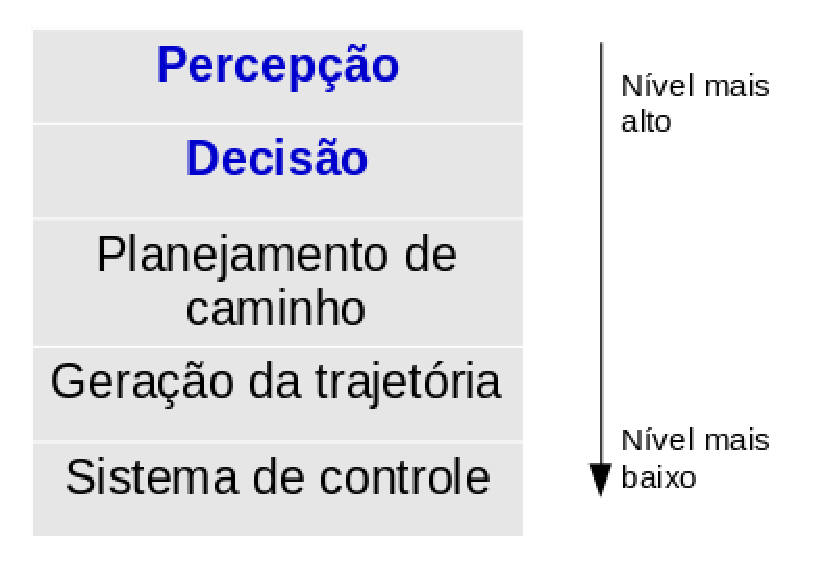
\includegraphics[scale=0.6]{figuras/camadas.eps}
	\caption[Arquitetura do robô]{Arquitetura do robô. Fonte \cite{vieira}.}
	\label{img:camadas}
\end{figure}

\section{Montagem do Robô}

	Esta seção tem como objetivo apresentar a forma de montagem do robô utilizada durante a pesquisa. O padrão utilizado foi escolhido após a análise e comparação da margem de erro presente em dois tipos de montagem. Durante a primeira etapa deste trabalho (TCC 1), foi utilizado o robô montado com esteiras para movimentação, seguindo o padrão encontrado em tanques de guerra, como pode ser observado na Figura \ref{img:montagem_antiga}.

	\begin{figure}[H]
		\centering
		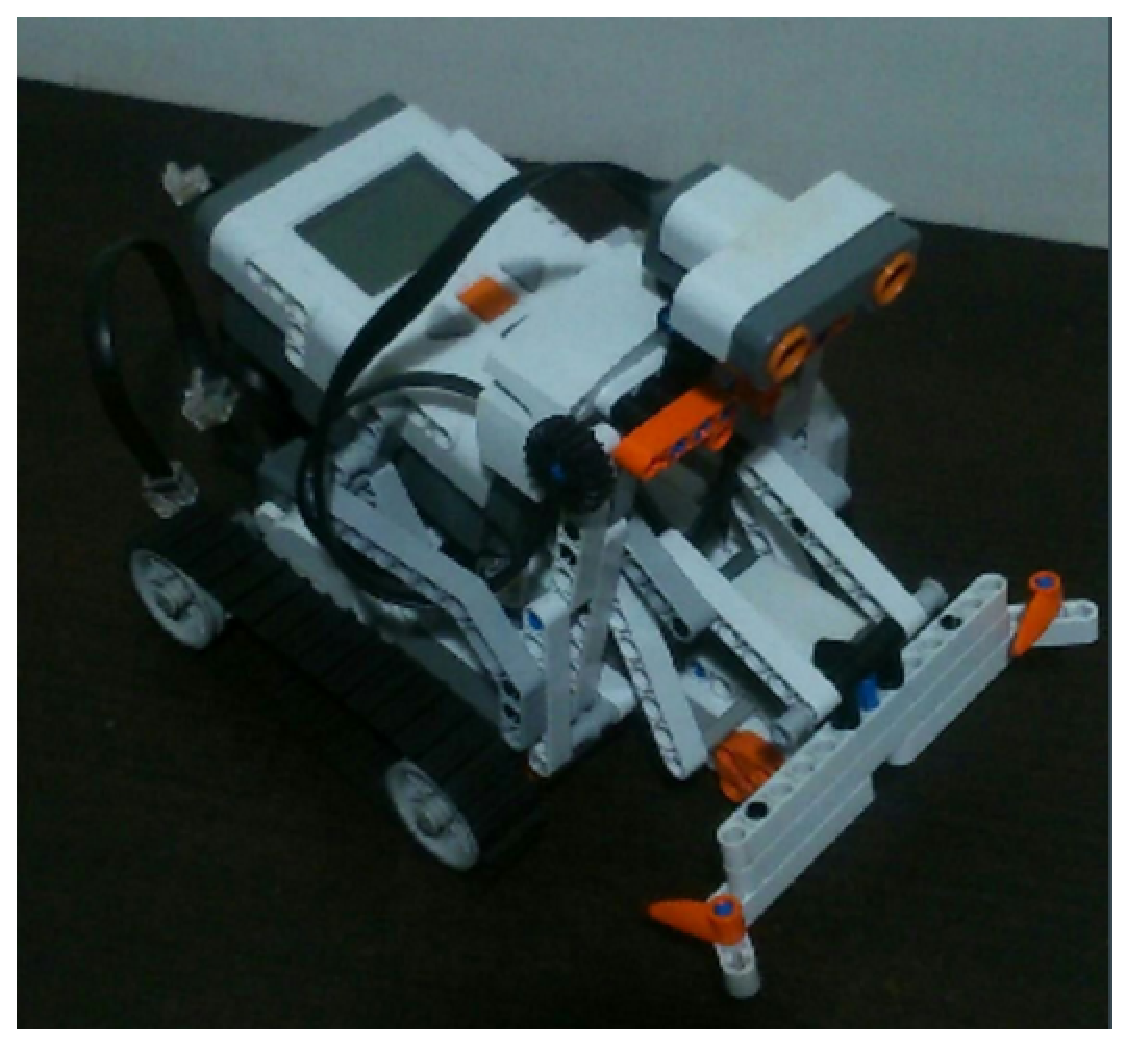
\includegraphics[scale=0.6]{figuras/montagem_antiga.eps}
		\caption[Montagem do Robô 1]{Montagem do Robô durante o TCC 1}
		\label{img:montagem_antiga}
	\end{figure}

	Porém, após algumas análises e pesquisas, concluiu-se que a utilização de esteiras maximiza a margem de erro durante a navegação, prejudicando a qualidade do movimento. Isto se dá, segundo \cite{legonxj}, devido a área de contato entre a esteira e o chão. Quanto maior a área de contato, mais crítico é o resultado de derrapagens durante a movimentação, inviabilizando sua utilização para este objetivo. Desse modo, a partir da segunda etapa desta pesquisa, passou-se a utilizar um robô do tipo \textit{Carpet} (de acordo com a nomenclatura da LEGO), onde estão presentes duas rodas motorizadas e uma terceira roda para equilíbrio do robô.

	Além do padrão relacionado as rodas, deve-se atentar a localização do sensor de distância. Este deve estar localizado exatamente no centro do robô, ou o mais próximo disso. As Figuras \ref{img:montagem_robo}  e \ref{img:montagem_robo_costas} apresentam o robô utilizado durante a segunda etapa desta pesquisa.

	\begin{figure}[H]
		\centering
		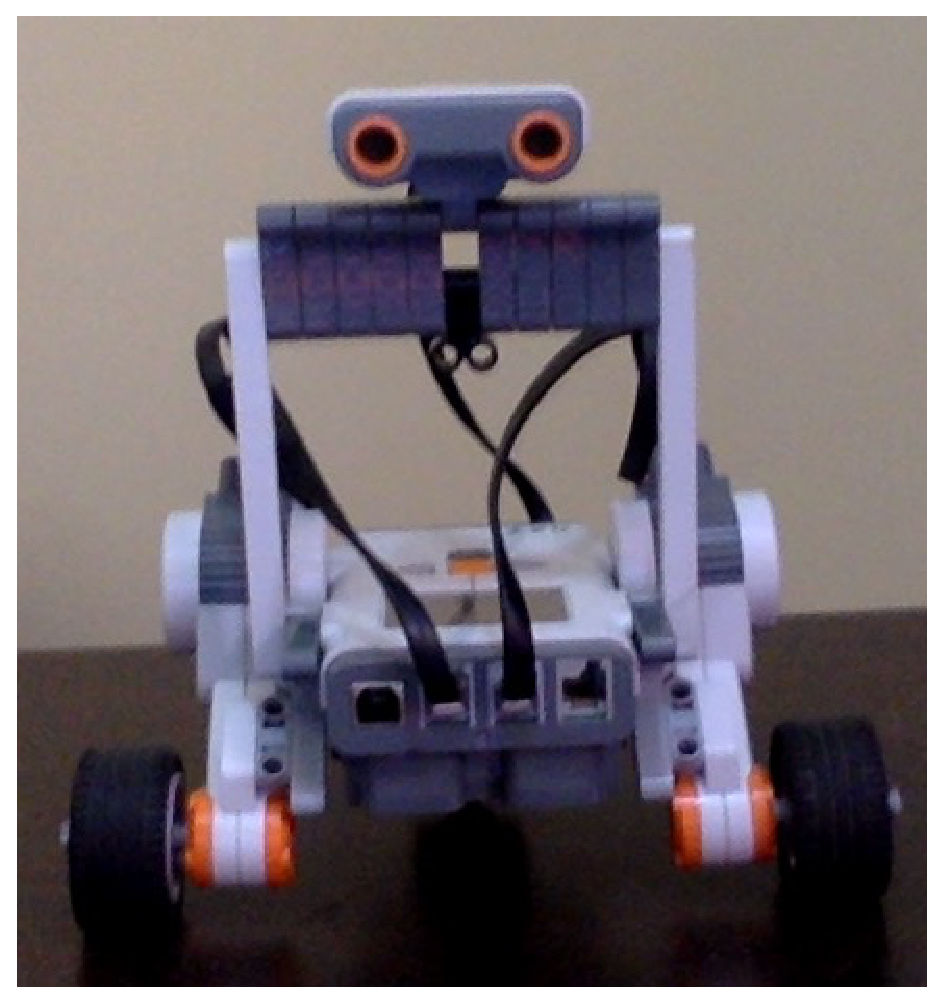
\includegraphics[scale=0.7]{figuras/frente.eps}
		\caption[Montagem do Robô 2]{Montagem do Robô durante o TCC 2 - Frente}
		\label{img:img:montagem_robo}
	\end{figure}

	A terceira roda, utilizada apenas como roda de apoio é feita a partir de uma simples montagem de peças LEGO, como pode ser observado na Figura \ref{img:montagem_robo_costas}.

	\begin{figure}[H]
		\centering
		\includegraphics[scale=0.3]{figuras/rodinha.eps}
		\caption[Montagem do Robô 3]{Montagem do Robô durante o TCC 2 - Roda de Apoio}
		\label{img:montagem_robo_costas}
	\end{figure}

	Em relação ao código utilizado durante a pesquisa, as portas utilizadas para acesso aos motores e sensores seguem o padrão apresentado na Tabela \ref{tab:portas_motores_sensores}.

	\begin{table}[H]
		\centering
		\caption{Configuração dos componentes utilizados}
		\label{tab:portas_motores_sensores}
		\begin{tabular}{|c|c|}
		\hline
		\textbf{Porta} & \textbf{Componente} \\ \hline
		B              & Motor esquerdo      \\ \hline
		C              & Motor direito       \\ \hline
		S1             & Sonar               \\ \hline
		\end{tabular}
	\end{table}

\section{Ambiente de Navegação}

	Esta seção tem como objetivo apresentar o ambiente de navegação utilizado durante a realização da pesquisa. Ao longo da mesma, diversos ambientes foram utilizados, possibilitando a escolha da melhor configuração para análise efetiva dos resultados.

	Sabe-se que, independente do piso selecionado, erros estarão presentes, seja devido a deslizes entre as rodas e o piso, ou devido a margem de erro presente nos sensores odométricos. Desse modo, buscou-se selecionar um piso que possibilite uma margem de erro mínima, dentre as opções presentes em um contexto simplificado, de uma escola, por exemplo.

	Deve-se optar sempre por pisos lisos, ou seja, sem irregularidades, as quais podem 'travar' a roda de apoio, que não possui um formato tão adequado quanto as rodas motorizadas. Este formato diferenciado da roda de apoio, o qual pode ser visualizado na Figura \ref{img:montagem_robo_costas}, pode gerar diversas interferências durante a navegação, principalmente em pisos que possuem 'rachaduras', como as presentes em pisos feitos com azulejo, por exemplo.

	Devido a esta característica da roda de apoio, pisos feitos com azulejo devem ser evitados, optando sempre por pisos tão lisos quanto possível. Um exemplo do piso utilizado durante esta pesquisa pode ser visualizado na Figura \ref{img:piso_ambiente}.

	\begin{figure}[H]
		\centering
		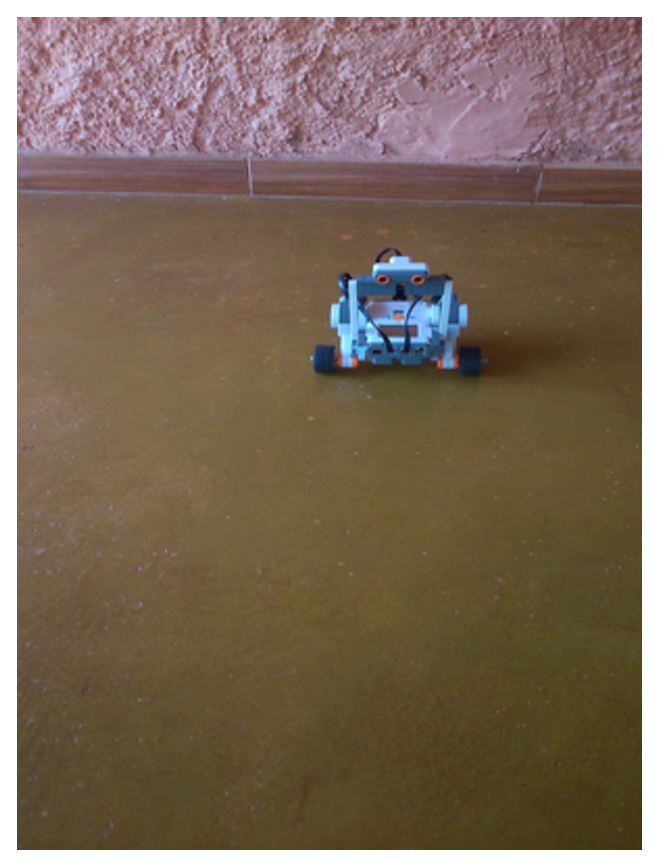
\includegraphics[scale=0.8]{figuras/piso_ambiente.eps}
		\caption[Exemplo de piso]{Exemplo de piso.}
		\label{img:piso_ambiente}
	\end{figure}

	Com o piso definido, deve-se definir o padrão de obstáculos no ambiente. Como o objetivo desta pesquisa é analisar a viabilidade da utilização de técnicas de auto-localização e mapeamento de ambientes em robôs simples, utilizando apenas um sensor de distância do tipo \textit{sonar}, deve-se adequar o padrão de obstáculos no ambiente, buscando minimizar a margem de erro presente na análise.

	Como o robô utiliza obstáculos para se auto-localizar, tratando os obstáculos como \textit{pontos de referência}, os mesmos precisam se adequar ao máximo as características presentes nos sonares. A principal característica do sonar utilizado é apresentada na Figura \ref{img:cone}, a qual envolve o modelo de emissão do sinal utilizado pelo sonar.

	Para que um sonar funcione, o mesmo emite um sinal que irá refletir no primeiro obstáculo encontrado, retornando ao robô e, a partir da análise do tempo gasto para percorrer este caminho, chega-se a conclusão da distância entre o robô e o objeto que refletiu o sinal. Porém, este sinal não é emitido de forma unidimensional, sua emissão é feita no formato de cone, devido as características físicas relacionadas a tramissão do som no ar. Por esse motivo, alguns erros podem ser adicionados à solução, visto que em determinadas situações, o objeto que refletiu o sinal sonoro não se encontra exatamente à frente do robô.

	Isto significa que o robô pode enxergar obstáculos mesmo quando não existe nenhum obstáculo diretamente à sua frente, enxergando obstáculos presentes nas laterais e tratando-os como obstáculos frontais. Infelizmente não existe uma solução exata para solucionar este problema, enquanto for utilizado um sonar para detecção de distâncias, este problema existirá.
	Desse modo, buscando minimizar a taxa de ocorrência desse \textit{'engano'}, o ambiente foi pensado e criado utilizando paredes lisas e em formatos uniformes, retilíneos.

	Como o objetivo da pesquisa é analisar a possibilidade da auto-localização dentro de um ambiente, optou-se pela não utilização de obstáculos entre as paredes. Fazendo com que o ambiente seja composto apenas de piso e paredes, como apresenta a Figura \ref{img:ambiente_utilizado}.

	Como o robô deverá analisar os pontos de referência (paredes) e a partir de determinadas características e se auto-localizar em relação ao mapa, o ambiente utilizado não pode ser simétrico. Ou seja, deve-se evitar a utilização de ambientes quadrados ou retangulares, por exemplo, já que o robô não conseguiria identificar características únicas em cada local do ambiente.
	A Figura \ref{img:exemplo_ambiente} apresenta uma boa opção de ambiente a ser utilizado, já que o mesmo possui características que viabilizam a comparação e conclusão de unicidade.

	\begin{figure}[H]
		\centering
		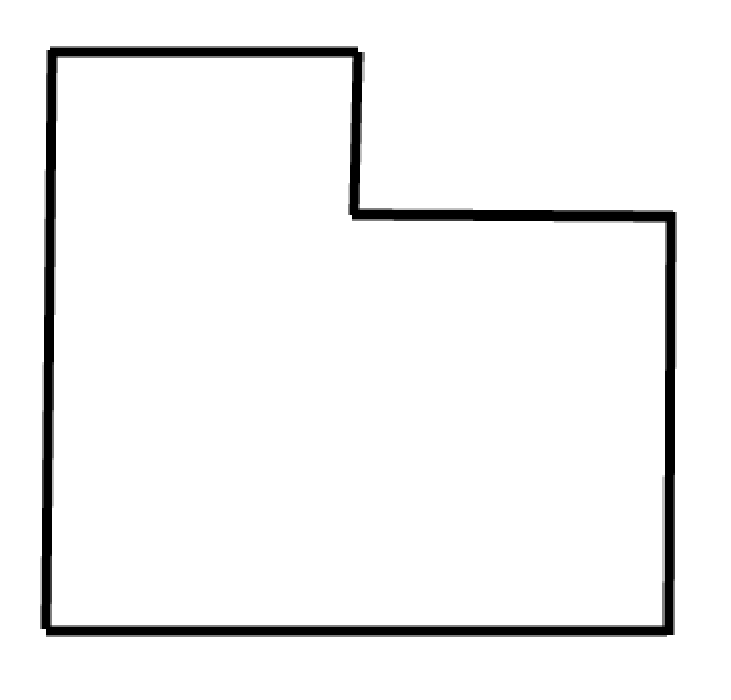
\includegraphics[scale=0.5]{figuras/exemplo_ambiente.eps}
		\caption[Exemplo de ambiente]{Exemplo de ambiente.}
		\label{img:exemplo_ambiente}
	\end{figure}

\section{Configuração e Integração das Tecnologias}

Nesta seção será apresentado o passo a passo para configuração e integração das tecnologias utilizadas durante este trabalho. A principal tecnologia utilizada é o pacote leJOS (Lego Java Operating System) NXJ, o qual possibilita a utilização da linguagem Java para implementação dos algoritmos durante a realização do trabalho. leJOS NXJ envolve um ambiente Java, um \textit{firmware} e uma API.

O ambiente java disponibilizado pelo leJOS NXJ possibilita integração com a IDE Eclipse, facilitando o \textit{upload} de códigos, atualização de \textit{firmware} e utilização da API. O \textit{firmware} é necessário pois cria uma máquina virtual Java no NXT, possibilitando a execução de códigos Java no \textit{Brick}. Além disso, a API leJOS envolve uma variedade de classes e métodos com algoritmos já desenvolvidos e disponibilizados para utilização durante o desenvolvimento. Com a utilização da API, o desenvolvedor não se preocupa com a implementação de algoritmos comuns, como de navegação e obtenção de dados dos sensores.

A plataforma leJOS NXJ é multiplataforma, possibilitando sua utilização no \textit{Windows}, \textit{Linux} e \textit{MAC OS}, nas seções abaixo estão descritos os passos para instalação e configuração do leJOS NXJ nas três plataformas.

\subsection{Instalação no Windows} % (fold)
\label{sub:instalação_no_windows}

	Primeiramente, para possibilitar a comunicação entre o PC e o NXT, deve-se instalar um \textit{USB Driver}, o qual pode ser encontrado \href{https://www.lego.com/en-us/mindstorms/downloads}{aqui}, optando pela versão de seu Brick (no caso deste trabalho, o NXT). Após a instalação do USB Driver, deve-se instalar o JDK (Java Development Kit) versão 1.8, disponivel \href{http://www.oracle.com/technetwork/java/}{aqui}.

	Após a instalação do JDK, deve-se indicar as variáveis de ambiente do Java, adicionando o caminho do diretório do JDK instalado no \textit{PATH}. Para isso, siga os seguintes passos:

	\begin{enumerate}
		\item Clique em iniciar
		\item Painel de controle
		\item Sistema
		\item Configurações avançadas
		\item Clique na tab Avançado
		\item Variáveis de Ambiente
		\item Procure a variável JAVA\_HOME (Se não existir, crie uma)
		\item Edite a variável PATH e adicione o seguinte ao valor da mesma: \textit{$\%java\_home\% \textbackslash$ bin}
	\end{enumerate}

	Feito isto, basta testar se o Java está funcionando. Para isso, abra o \textit{Command Prompt} (CMD) e exeute o comando \textit{java}, caso esteja funcionando, será apresentado algumas opções de utilização do comando \textit{java}.

	Agora que o Java já se encontra instalado e funcionando, basta instalar o NXJ, o qual se encontra \href{http://www.lejos.org/}{aqui}. Baixe o arquivo \textit{Setup.exe}, execute o arquivo e siga os comandos de instalação apresentados pelo próprio instalador. Ao final da instalação, será executado um programa para \textit{upload} de um novo \textit{firmware} para o NXT. Feito isto, o leJOS já se encontra instalado e funcionando.
% subsection instalação_no_windows (end)

\subsection{Instalação no Linux} % (fold)
\label{sub:instalação_no_linux}

	Seguindo a mesma lógica de instalação apresentada na seção anterior, primeiramente deve-se instalar o USB Driver e o JDK. Por motivo de organização, apresenta-se primeiramente os passos de instalação do JDK, seguido do USB Driver.

	Para instalar o JDK, baixe a última versão do JDK disponível \href{http://www.oracle.com/technetwork/java/}{aqui}. Instale o JDK, de acordo com sua distribuição linux, e edite o PATH, adicionando o caminho do /bin do JDK instalado utilizando a variável \textit{$\%java\_home\% \textbackslash$ bin}. Para verificar se a instalação e configuração foram feitas corretamente, execute o comando \textit{java} no terminal e observe se informações de utilização do comando são apresentadas.

	Siga os seguintes passos para preparar e instalar o USB Driver:

	\begin{enumerate}
		\item Instale a lib \textit{libusb}, disponível \href{http://libusb.sourceforge.net}{aqui}, para que as ferramentas do leJOS possam acessar as portas USB do PC.
		\item  Tenha certeza que você possui acesso de leitura e escrita no dispositivo NXT USB. Para isso, verifique o arquivo /dev/bus/usb (especificidades em cada distribuição linux).
		\item Use regras Udev. Para isto, crie um arquivo chamado \textit{/etc/udev/rules.d/70-lego.rules} e adicione o seguinte conteúdo no mesmo:

		\begin{lstlisting}
			# Lego NXT brick in normal mode
			SUBSYSTEM=="usb", DRIVER=="usb",
			ATTRS{idVendor} == "0694",
			ATTRS{idProduct} == "0002", GROUP="lego",
			MODE = "0660"

			#Lego NXT brick in firmware update mode (Atmel SAM-BA mode)

			SUBSYSTEM == "usb", DRIVER == "usb",
			ATTRS{idVendor} == "03eb",
			ATTRS{idProduct} == "6124", GROUP="lego",
			MODE = "0660"
		\end{lstlisting}
	\end{enumerate}

	Feito isto, basta instalar o leJOS NXJ, de acordo com os passos a seguir:

	\begin{enumerate}
		\item Baixe o arquivo \textit{tar.gz} \href{www.lejos.org}{aqui}.
		\item Descompacte o arquivo no diretório \textit{/opt/lejos\_nxj/}.
		\item Crie a variável de ambiente \textit{NXJ\_HOME} apontando para o diretório onde foi descompactado o leJOS.
		\item Adicione o diretório \textit{/bin} da variável \textit{NXJ\_HOME} no seu \textit{PATH}.
		\item Caso tenha problema com permissões, deve alterar as permissões de execução neste diretório.
		\item Seu \textit{PATH} deve conter também o caminho para o binário \textit{ant}.
		\item Agora basta gerar a distribuição. Troque para o diretório de criação e rode \textit{ant}.
	\end{enumerate}

	Feito isto, basta atualizar o \textit{firmware} no seu NXT.
% subsection instalação_no_linux (end)

\subsection{Instalação no MAC OS} % (fold)
\label{sub:instalação_no_mac_os}

	Primeiramente deve-se instalar o JDK no sistema, fazendo download do mesmo \href{http://www.oracle.com/technetwork/java/}{aqui}. Instale o JDK e edite o PATH, adicionando o caminho do /bin do JDK instalado utilizando a variável \textit{$\%java\_home\% \textbackslash$ bin}. Para verificar se a instalação e configuração foram feitas corretamente, execute o comando \textit{java} no terminal e observe se informações de utilização do comando são apresentadas.

	Para instalar o leJOS no MAC OS, deve-se primeiro configurar o ambiente, de acordo com os seguintes passos:

	\begin{enumerate}
		\item Instale o Software LEGO, o qual irá instalar também os Drivers USB.
		\item Baixe o instalador \href{www.lejos.org}{aqui}.
		\item Extraia os arquivos para uma nova localização, como \textit{/Applications/lejos\_nxj}.
		\item Se você utiliza o login de administrador, você precisa criar (ou editar) o arquivo \textit{.tcshrc} no seu diretório \textit{home}.
		\item Adicione as seguintes linhas no diretório onde o leJOS foi extraído:
		\begin{lstlisting}
			setenv NXJ_HOME /Applications/lejos_nxj
			setenv PATH ${PATH}:${NXJ_HOME}/bin
		\end{lstlisting}
		\item Salve o arquivo em \textit{/users/administrator}.
		\item Abra um terminal e execute \textit{tcsh}, você verá o tcsh shell.
		\item Execute \textit{setenv} para ter certeza que as variáveis de ambiente estão setadas corretamente.
	\end{enumerate}
% subsection instalação_no_mac_os (end)

\subsection{Utilizando leJOS NXJ} % (fold)
\label{sub:utilizando_lejos_nxj}

	Após a instalação do leJOS, apresentada nas seções anteriores, tudo está pronto para desenvolvimento e utilização das ferramentas presentes no pacote. Esta seção tem como objetivo apresentar as formas de utilização do pacote.

	O USB é a única forma de \textit{upar} o \textit{firmware} para o seu NXT. Para isto, pode-se utilizar o modo gráfico, o modo por linha de comando do terminal ou até o modo de integração com a IDE Eclipse. Para fazê-lo, siga os passos:

	\begin{enumerate}
		\item Conecte seu NXT ao PC via USB.
		\item Execute o arquivo \textit{nxj-flashg}, presente no diretório \textit{/bin} do leJOS para utilizar o modo gráfico, ou apenas execute \textit{nxjflash}.
		\item No modo gráfico clique em \textit{upload firmware} e aguarde alguns instantes até que o processo seja concluído. Não retire o NXT durante o \textit{upload} do \textit{firmware}.
	\end{enumerate}

	Feito isso, seu NXT está pronto para executar código Java.
% subsection utilizando_lejos_nxj (end)

\subsubsection{Conflitos de tecnologias e soluções}

A tecnologia leJOS é utilizada, em sua grande maioria, por pesquisadores e estudantes interessandos no contexto de Robótica. Desse modo, interessados na tecnologia
podem ainda utilizar e pesquisar conceitos em outras tecnologias, como o Arduino, por exemplo.

Desse modo, esta seção tem como objetivo apresentar um possível problema encontrado durante a utilização do leJOS por pesquisadores e/ou estudantes que também
costumam utilizar a tecnologia Arduino. Os \textit{drivers} utilizados para acesso do NXT por parte do computador podem conflitar com os \textit{drivers} utilizados
para o mesmo propósito na tecnologia Arduino, principalmente ao utilizar o Sistema Operacional Windows. Este conflito pode gerar falhas na comunicação, impossibilitando
o \textit{upload} de \textit{firmware} e códigos do computador ao NXT.

Para solucionar este problema, pode-se simplesmente desinstalar o \textit{software} do Arduino ou, caso deseje trabalhar com as duas tecnologias, deve-se realizar os seguintes passos:

\begin{enumerate}
	\item Desconectar o computador da Internet;
	\item Abrir o gerenciador de dispositivos (Botão direito em "Meu Computador");
	\item Conectar o NXT via USB (O gerenciador de dispositivos será atualizado);
	\item Vá até Portas e selecione Bossman;
	\item Clique em "Atualizar Driver" e selecione a opção de "Atualização Manual";
	\item Selecione o Driver da Lego, dentre as opções disponíveis;
	\item Feito isto, basta realizar o \textit{upload} do \textit{firmware} ou código ao NXT.
\end{enumerate}


\subsection{Utilizando IDE Eclipse} % (fold)
\label{sub:utilizando_ide_eclipse}

	É possível utilizar a API leJOS e suas ferramentas utilizando apenas um editor de texto e comandos via terminal, porém o trabalho pode se tornar cansativo e
	desgastante, já que a implementação se torna lenta e ineficiente, assim como o processo de \textit{debug}. Para facilitar este processo, pode-se utilizar
	a IDE (\textit{Integrated Development Environment}) do Eclipse, possibilitando a implementação, compilação e upload de códigos e de \textit{firmware} para o NXT.

	A ferramenta Eclipse foi desenvolvida pela \href{https://www.ibm.com/br-pt/}{IBM} e hoje é a IDE mais utilizada para desenvolvimento Java em todo o mundo.
	Para utilizar a IDE Eclipse para a implementação dos códigos com a API leJOS, basta realizar os seguintes passos.

	\begin{enumerate}
		\item Faça download do Eclipse \href{www.eclipse.org}{aqui};
		\item Descompacte o arquivo no diretório permanente do Eclipse;
		\item Feito isso basta executar o arquivo eclipse;
		\item Com o Eclipse aberto, selecione Help > Install New Software;
		\item Em frente a caixa de dialógo apresentada, selecione a opção Add;
		\item Em Add, na opção Name digite "leJOS NXJ";
		\item Na localização digite: "http://lejos.sourceforge.net/tools/eclipse/plugin/nxj/";
		\item Clique em Ok e selecione o \textit{checkbox} do plugin, selecionando Next em seguida;
		\item Leia e aceite os termos da licença e clique em Next;
		\item Pronto! O plugin já se encontra instalado, agora basta reiniciar o Eclipse e utilizá-lo normalmente.
	\end{enumerate}

	Durante a implementação, caso seja necessária ajuda sobre determinado método ou classe, basta consultar os arquivos de Ajuda do leJOS, que se encontram em
	Help > Help Contents no Eclipse, na seção leJOS NXJ.

% subsection utilizando_ide_eclipse (end)
\section{Arquitetura da Solução}

\section{Considerações Parciais}
